\documentclass[11pt]{article}
\usepackage[a4paper,margin=1in]{geometry}
\usepackage{amssymb,mathtools}
\usepackage{booktabs}
\usepackage{graphicx}
\usepackage{subcaption}
\usepackage[T1]{fontenc}
\usepackage{lmodern}
\usepackage{float}
\usepackage[utf8]{inputenc}
\usepackage{hyperref}

\title{Comp 480/580 - Assignment \#2}
\author{Dev Sanghvi - \texttt{ds221}}
\date{Rice University \\ Date: 10/13/2025}

\begin{document}
\maketitle

\section*{Problem Overview}
This assignment compares three streaming sketch data structures, Count-Min, Count-Median, and Count-Sketch, on the heavy-hitter problem using the AOL query log. Words are tokenized from the \texttt{Query} column, inserted with unit weight into each sketch and into an exact dictionary, and then evaluated across multiple accuracy regimes. Building on Assignment~\#1, our MurmurHash-based hash family (with $d=5$ rows and range $R\in\{2^{10},2^{14},2^{18}\}$) feeds each sketch with pairwise-independent locations (and signs for Count-Sketch).

\section{Implementation Summary}
\begin{itemize}
  \item \textbf{Driver (\texttt{main\_a2.py})}: streams tokens from disk, updates all sketches, and maintains an exact dictionary for evaluation.
  \item \textbf{Sketches (\texttt{assignment2/sketches.py})}: implements Count-Min, Count-Median, and Count-Sketch using a shared hash family defined in \texttt{assignment2/hashing.py}. Each sketch supports \texttt{update()} and \texttt{estimate()}; Count-Sketch uses $\pm1$ signs when updating.
  \item \textbf{Top-$k$ tracker}: a small heap-backed structure keeps the best 500 frequent tokens per sketch; we feed Count-Median with its median estimate on every update, so the heap logic mirrors Count-Min and Count-Sketch exactly.
  \item \textbf{Outputs}: for each $R$, we produce error curves on three buckets (Frequent-100, Random-100, Infrequent-100) and a plot of the intersection size $|\text{Top-500}_\text{sketch}\cap\text{Top-100}_\text{truth}|$ versus $R$.
\end{itemize}

\section{Run Configuration}
All runs fix the random seed to \texttt{20251013} for reproducibility. The dataset is streamed sequentially and may be supplied explicitly.  Table~\ref{tab:run-summary} is auto-generated after each execution and records specifics corresponding to the last run which produced the current plots.

\begin{table}[H]
  \centering
  \caption{Run summary from latest execution}
  \label{tab:run-summary}
  \begin{tabular}{lr}
\toprule
Metric & Value \\
\midrule
Processed tokens & 9\,896\,118 \\
Unique tokens & 451\,514 \\
Dictionary size (MiB) & 48.678 \\
Row budget & All rows \\
Dataset flag & \texttt{--dataset~user-ct-test-collection-01.txt} \\
\bottomrule
\end{tabular}
\end{table}
The table above will then report the full dataset scale (roughly $10^7$ tokens, $4.5\times 10^5$ unique terms, and a $\sim$50~MiB dictionary footprint).

\section{Plots}
Figures~\ref{fig:error-r1024}--\ref{fig:error-r262144} visualise the relative-error profiles for each sketch and $R$ setting. Figure~\ref{fig:top500} reports the top-500 intersection curve used in the grading rubric. Each figure is regenerated automatically from the latest execution.

\noindent\textbf{Observations for $R=2^{10}$.}

\begin{figure}[H]
  \centering
  \begin{subfigure}[t]{0.32\linewidth}
    \centering
    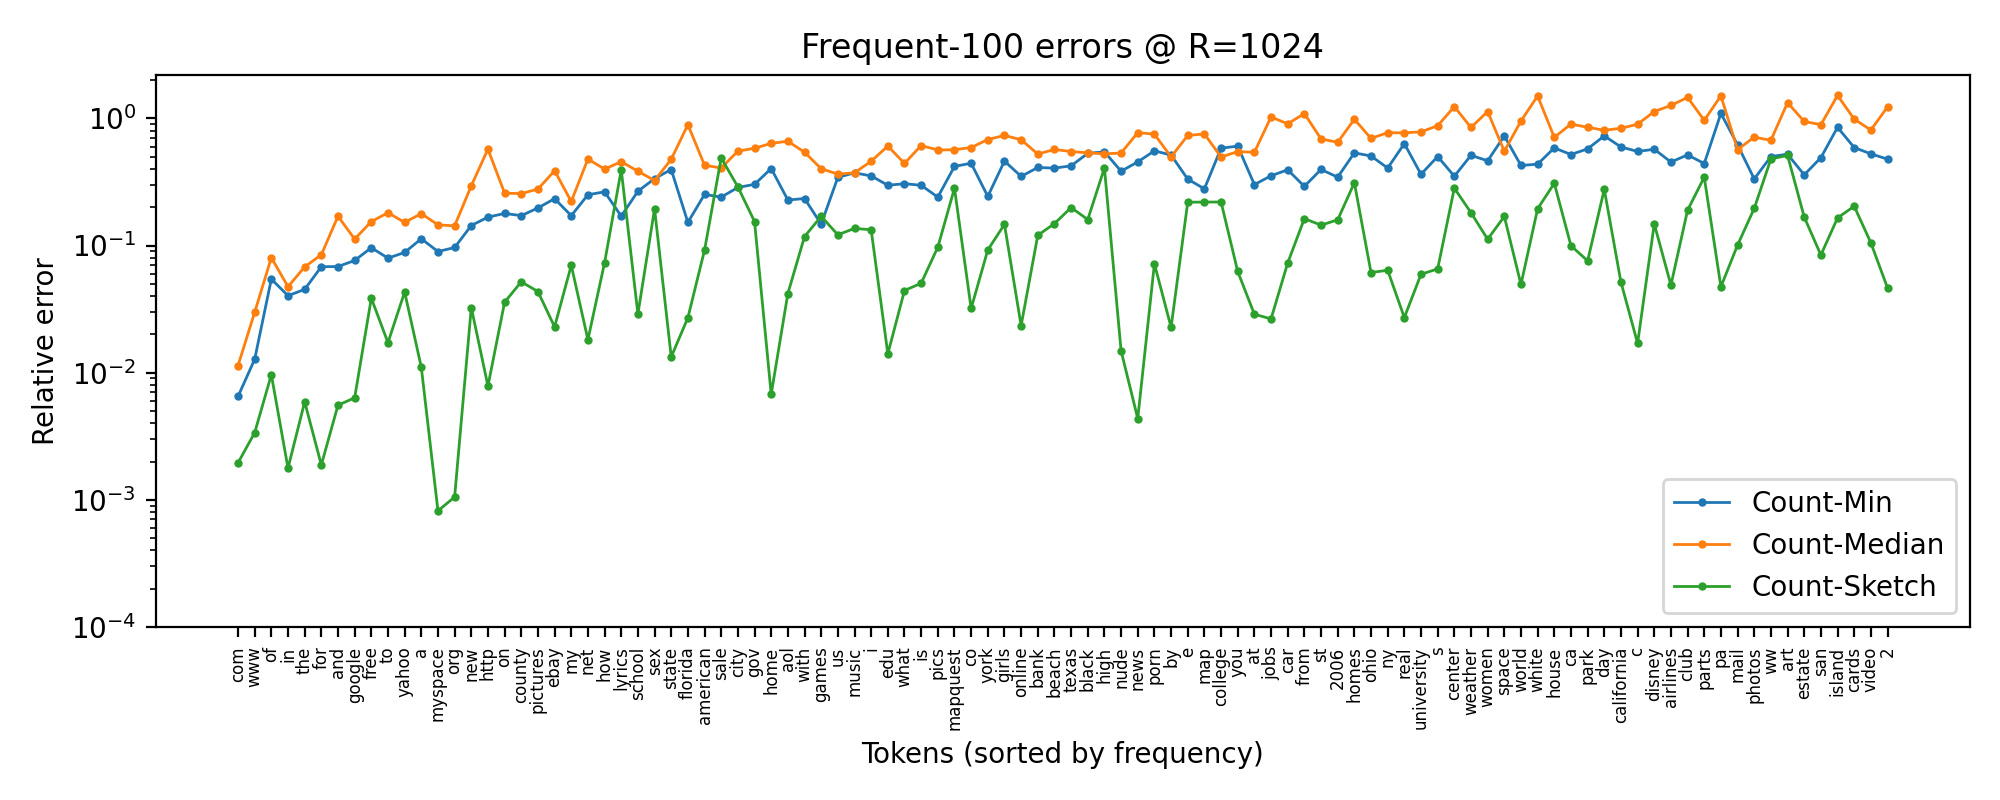
\includegraphics[width=\linewidth]{../outputs/a2/errors_R1024_Frequent_100.png}
    \caption{Frequent-100}
  \end{subfigure}
  \hfill
  \begin{subfigure}[t]{0.32\linewidth}
    \centering
    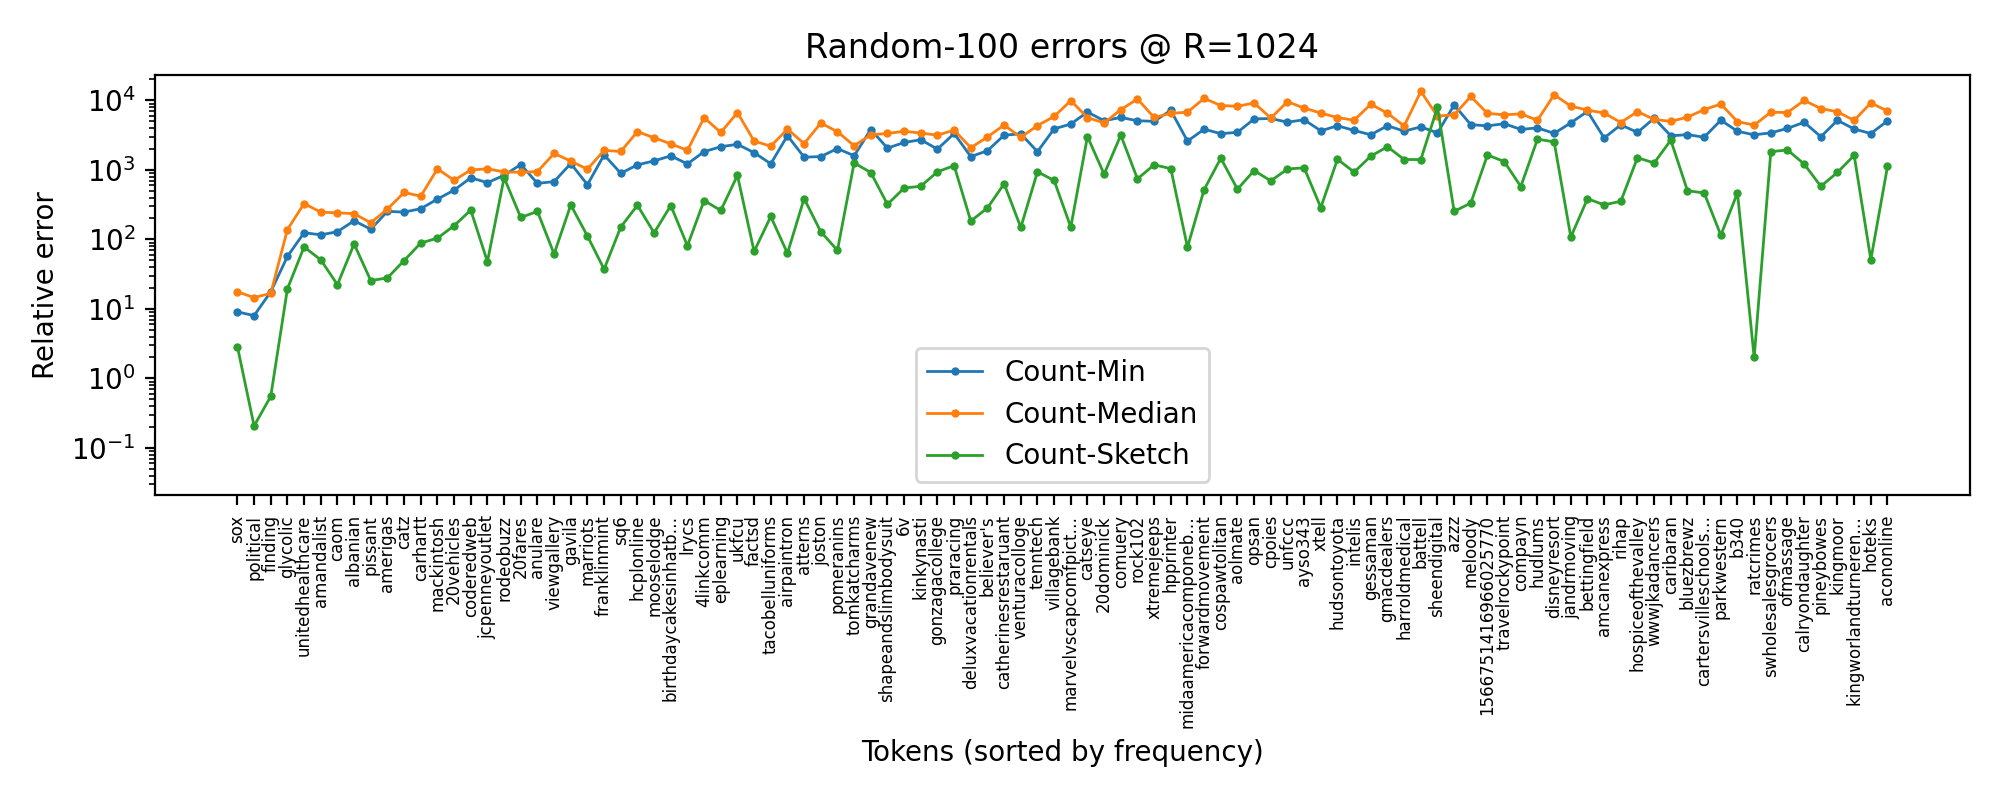
\includegraphics[width=\linewidth]{../outputs/a2/errors_R1024_Random_100.png}
    \caption{Random-100}
  \end{subfigure}
  \hfill
  \begin{subfigure}[t]{0.32\linewidth}
    \centering
    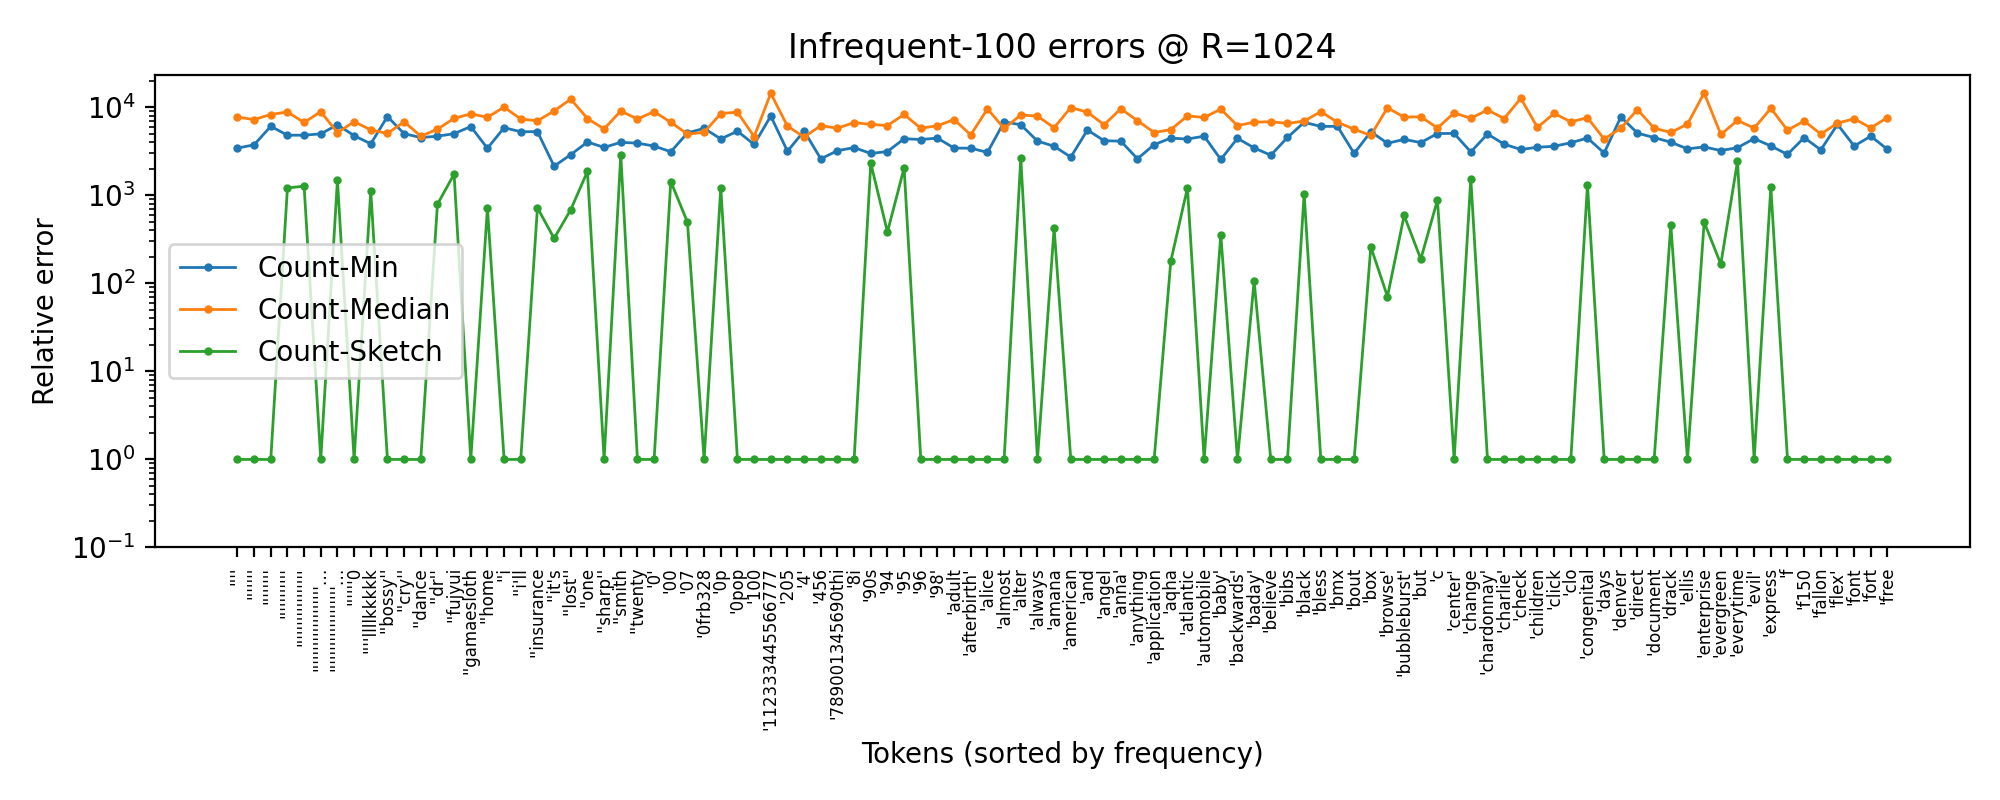
\includegraphics[width=\linewidth]{../outputs/a2/errors_R1024_Infrequent_100.png}
    \caption{Infrequent-100}
  \end{subfigure}
  \caption{Relative-error curves for $R=2^{10}$.}
  \label{fig:error-r1024}
\end{figure}



\begin{itemize}
  \item Frequent tokens already show a clear separation: Count-Min retains the smallest median error, Count-Median overshoots most often, and Count-Sketch sits between them.
  \item Random and infrequent tokens expose large positive bias in the sketches with unsigned counters, with Count-Median showing the steepest tails and Count-Sketch attenuating many of those errors via signed updates (Figures~\ref{fig:error-r1024}a--c).
\end{itemize}

\newpage

\noindent\textbf{Observations for $R=2^{14}$.}

\begin{figure}[H]
  \centering
  \begin{subfigure}[t]{0.32\linewidth}
    \centering
    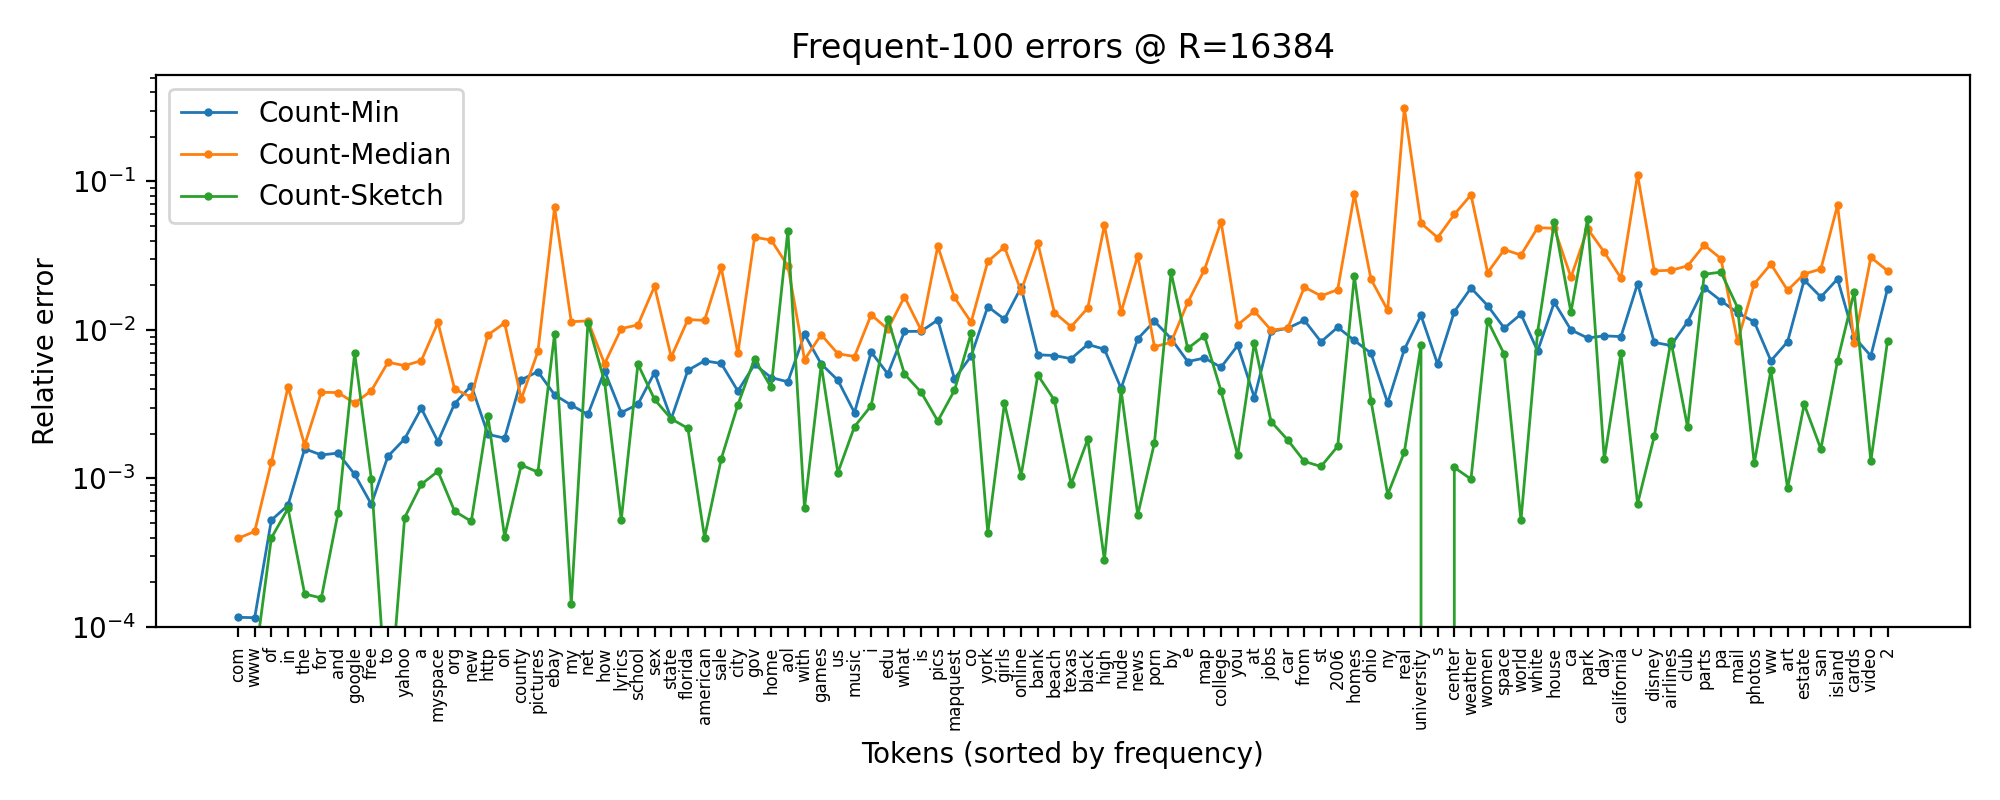
\includegraphics[width=\linewidth]{../outputs/a2/errors_R16384_Frequent_100.png}
    \caption{Frequent-100}
  \end{subfigure}
  \hfill
  \begin{subfigure}[t]{0.32\linewidth}
    \centering
    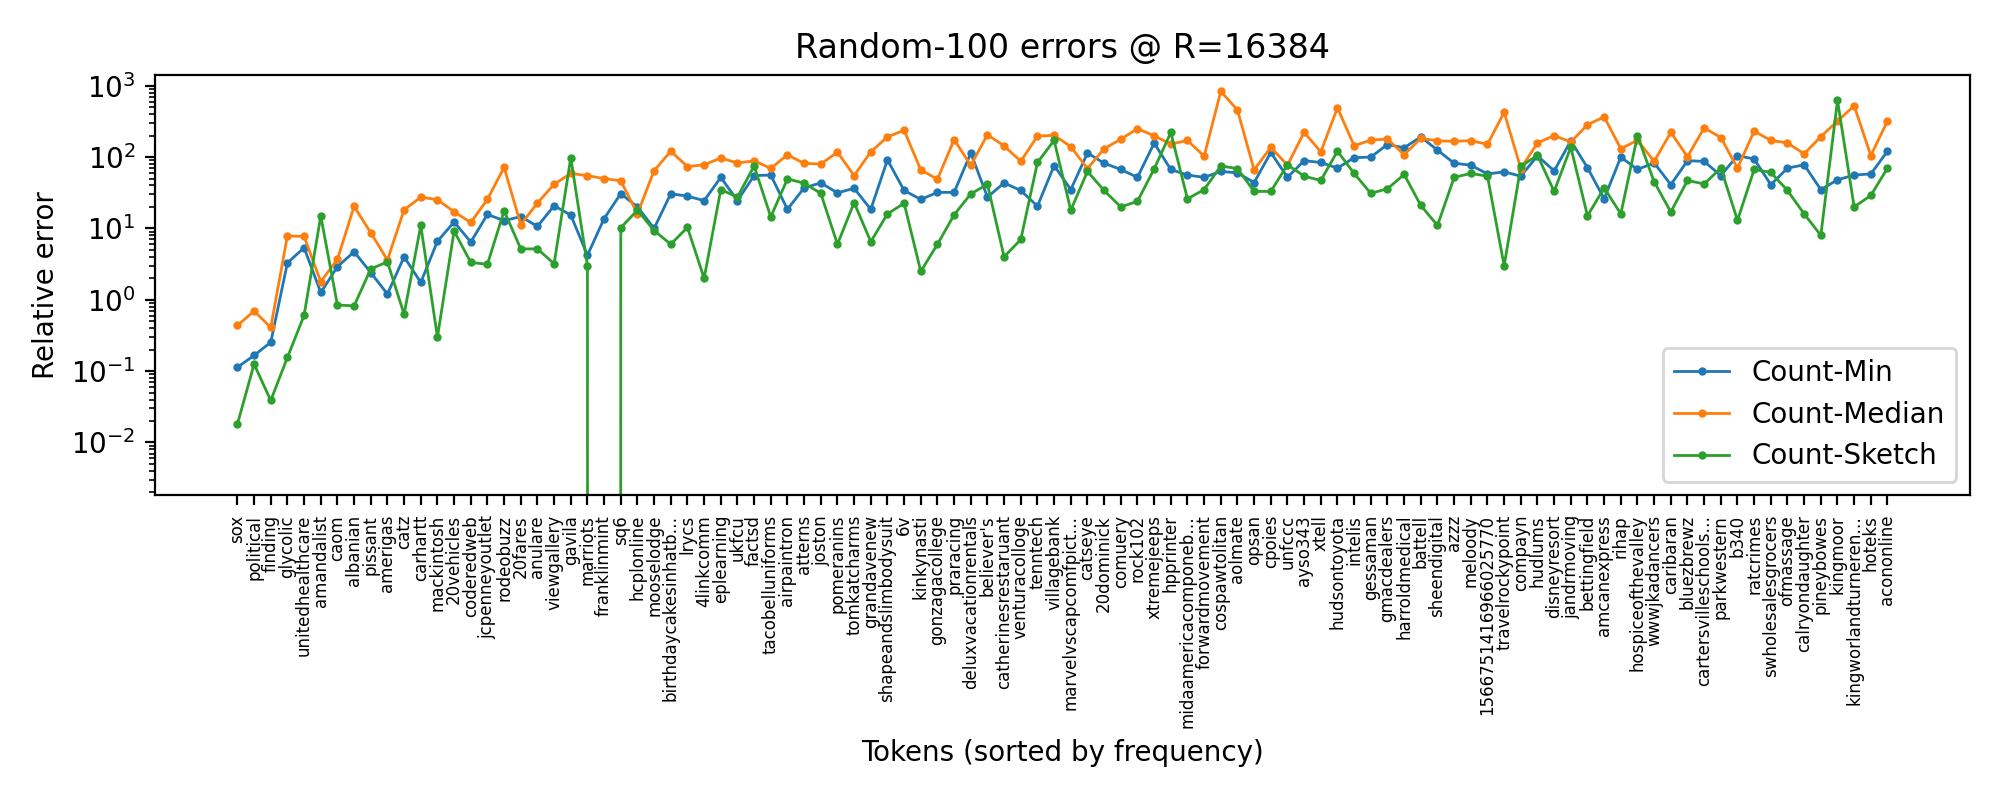
\includegraphics[width=\linewidth]{../outputs/a2/errors_R16384_Random_100.png}
    \caption{Random-100}
  \end{subfigure}
  \hfill
  \begin{subfigure}[t]{0.32\linewidth}
    \centering
    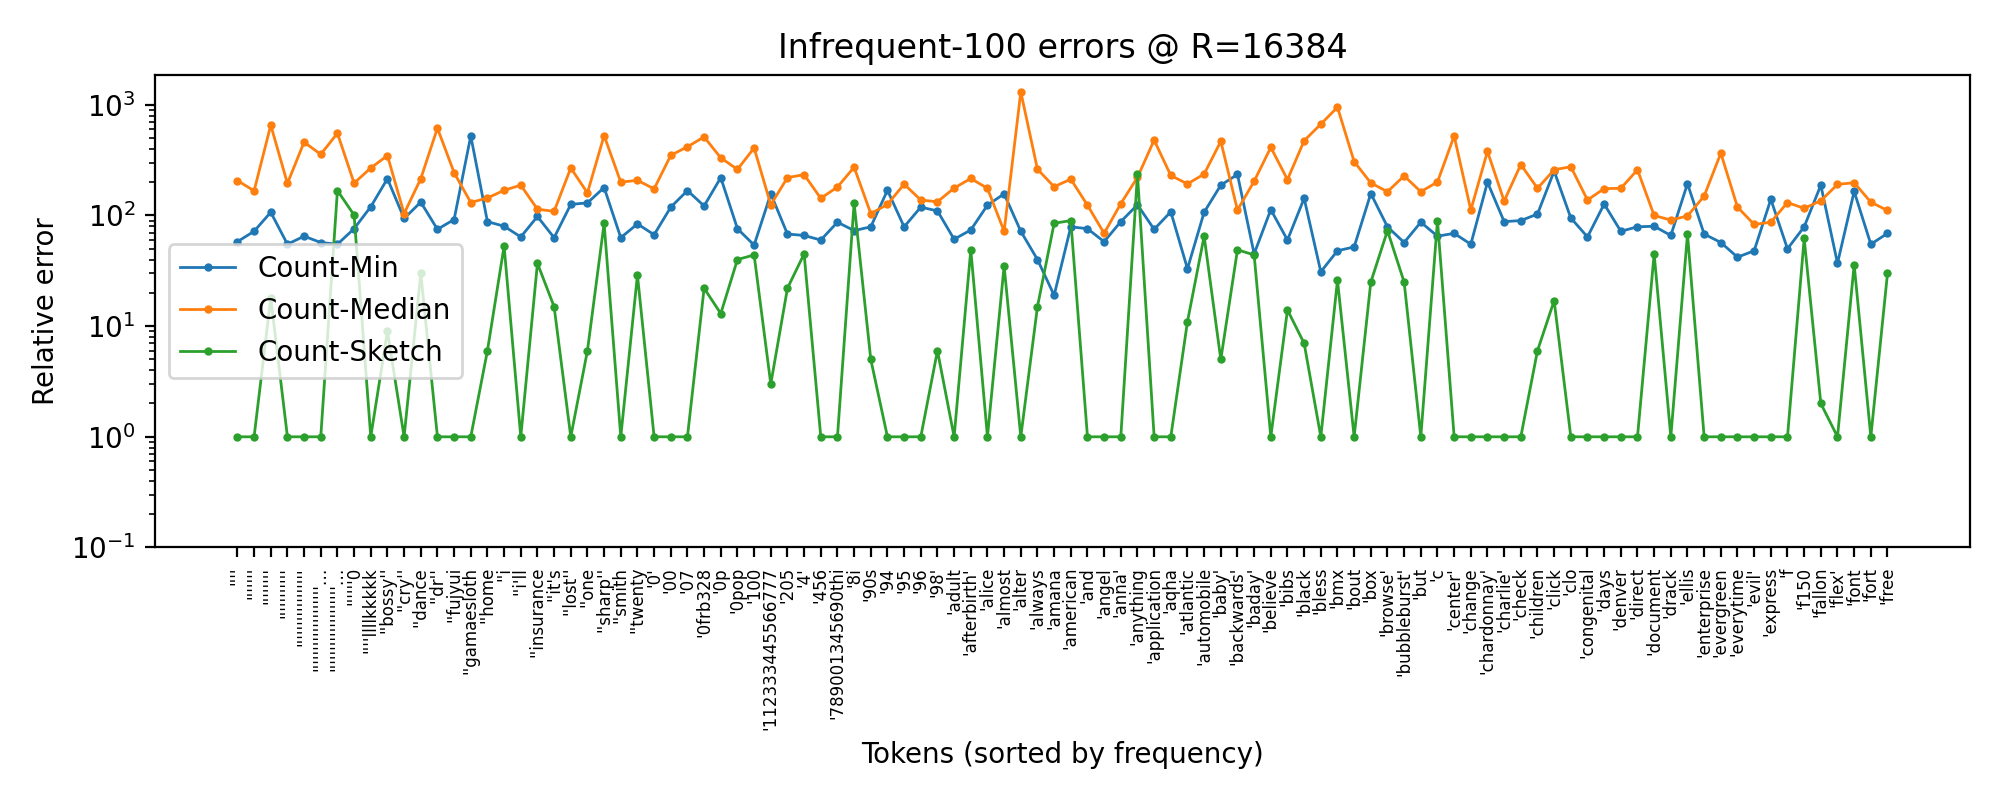
\includegraphics[width=\linewidth]{../outputs/a2/errors_R16384_Infrequent_100.png}
    \caption{Infrequent-100}
  \end{subfigure}
  \caption{Relative-error curves for $R=2^{14}$.}
  \label{fig:error-r16384}
\end{figure}



\begin{itemize}
  \item Median errors for all sketches collapse toward zero on Frequent-100 and Random-100 tokens (Table~\ref{tab:median-trends}, middle block), and even the infrequent bucket tightens considerably compared with $R=2^{10}$.
  \item The visual traces in Figure~\ref{fig:error-r16384} confirm that widening the sketch curbs most overestimation events for Count-Min and Count-Sketch; Count-Median still exhibits occasional spikes on rare tokens because its unsigned counters cannot cancel collisions.
\end{itemize}

\noindent\textbf{Observations for $R=2^{18}$.}

\begin{figure}[H]
  \centering
  \begin{subfigure}[t]{0.32\linewidth}
    \centering
    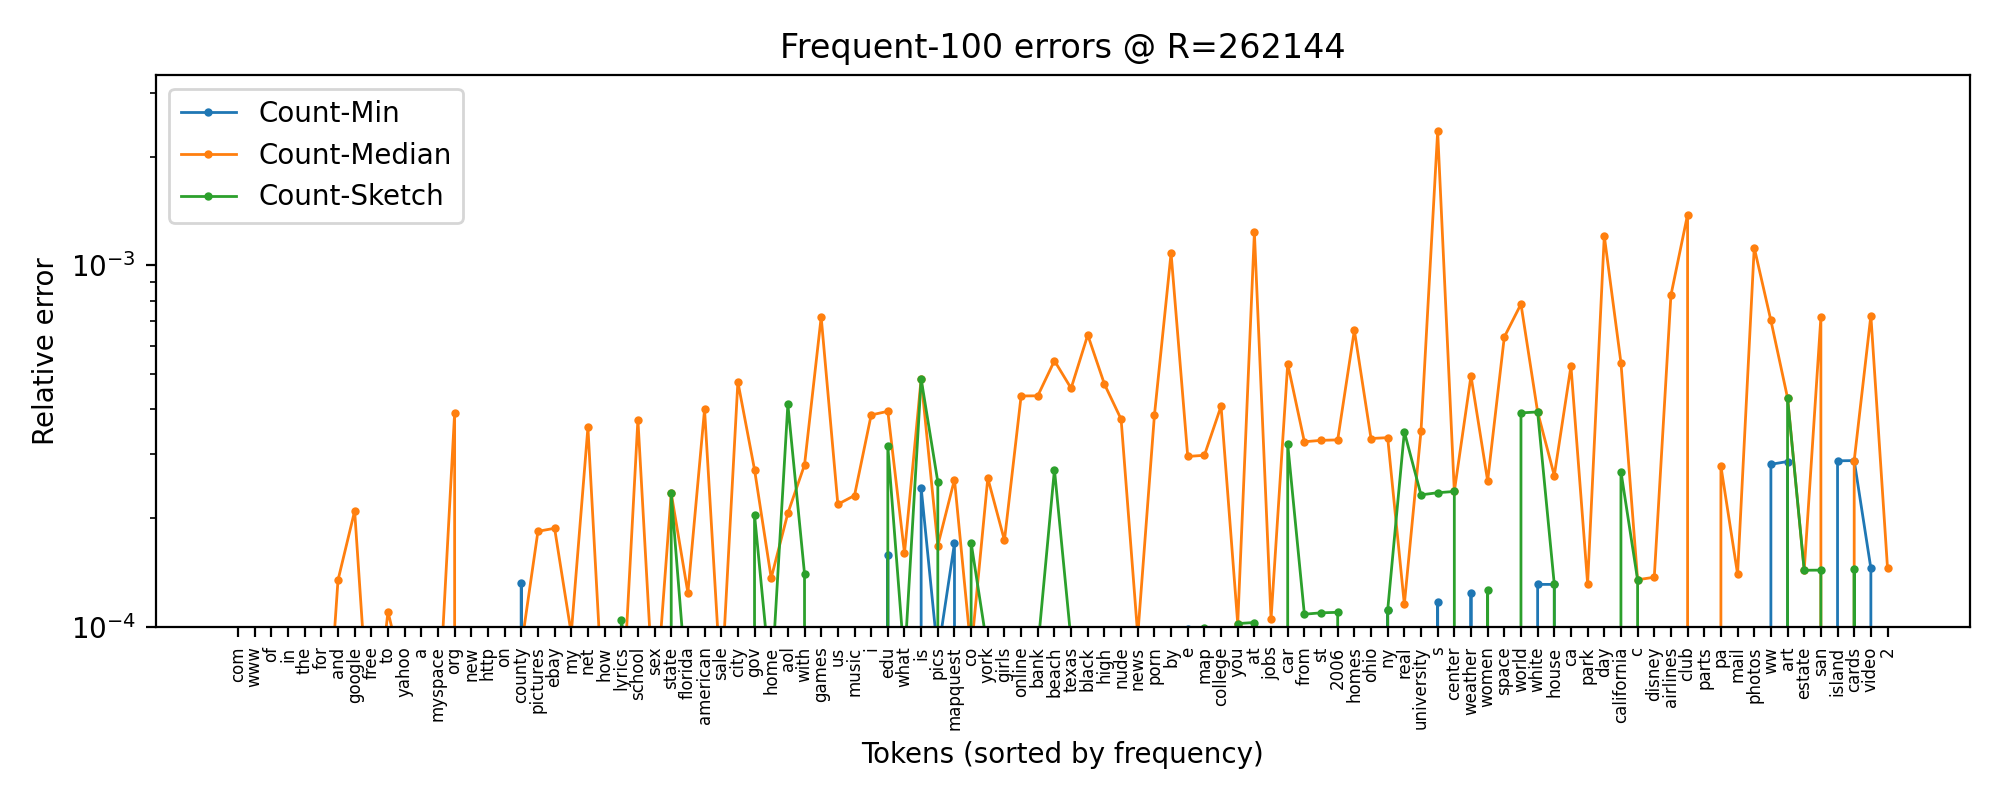
\includegraphics[width=\linewidth]{../outputs/a2/errors_R262144_Frequent_100.png}
    \caption{Frequent-100}
  \end{subfigure}
  \hfill
  \begin{subfigure}[t]{0.32\linewidth}
    \centering
    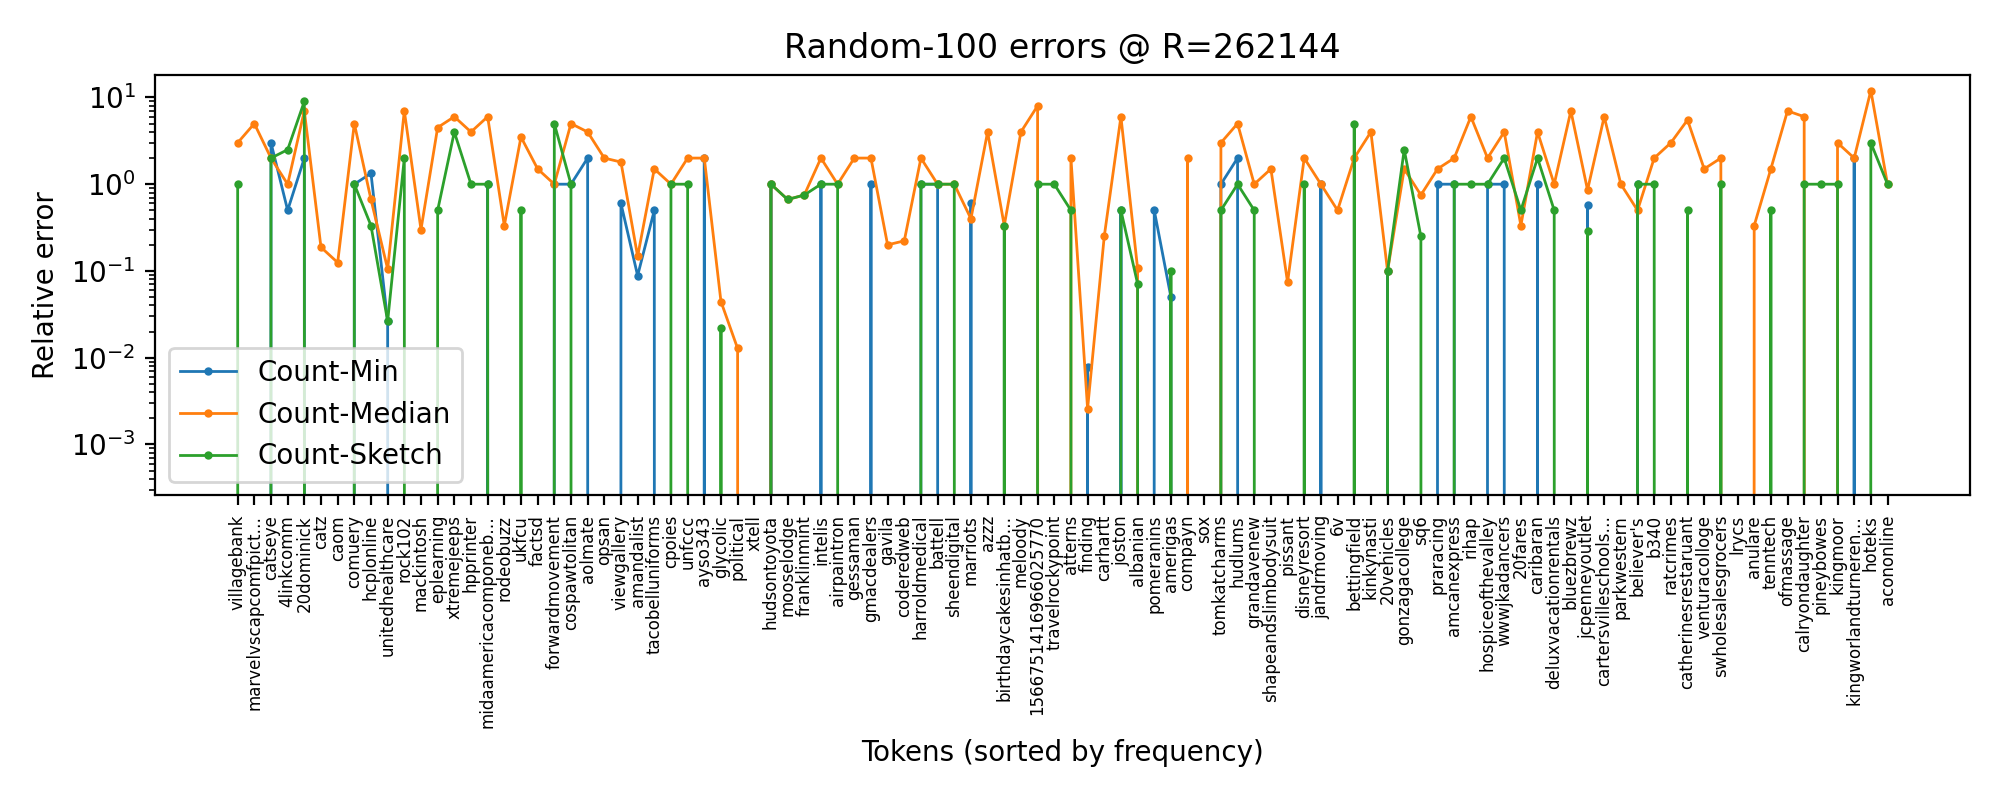
\includegraphics[width=\linewidth]{../outputs/a2/errors_R262144_Random_100.png}
    \caption{Random-100}
  \end{subfigure}
  \hfill
  \begin{subfigure}[t]{0.32\linewidth}
    \centering
    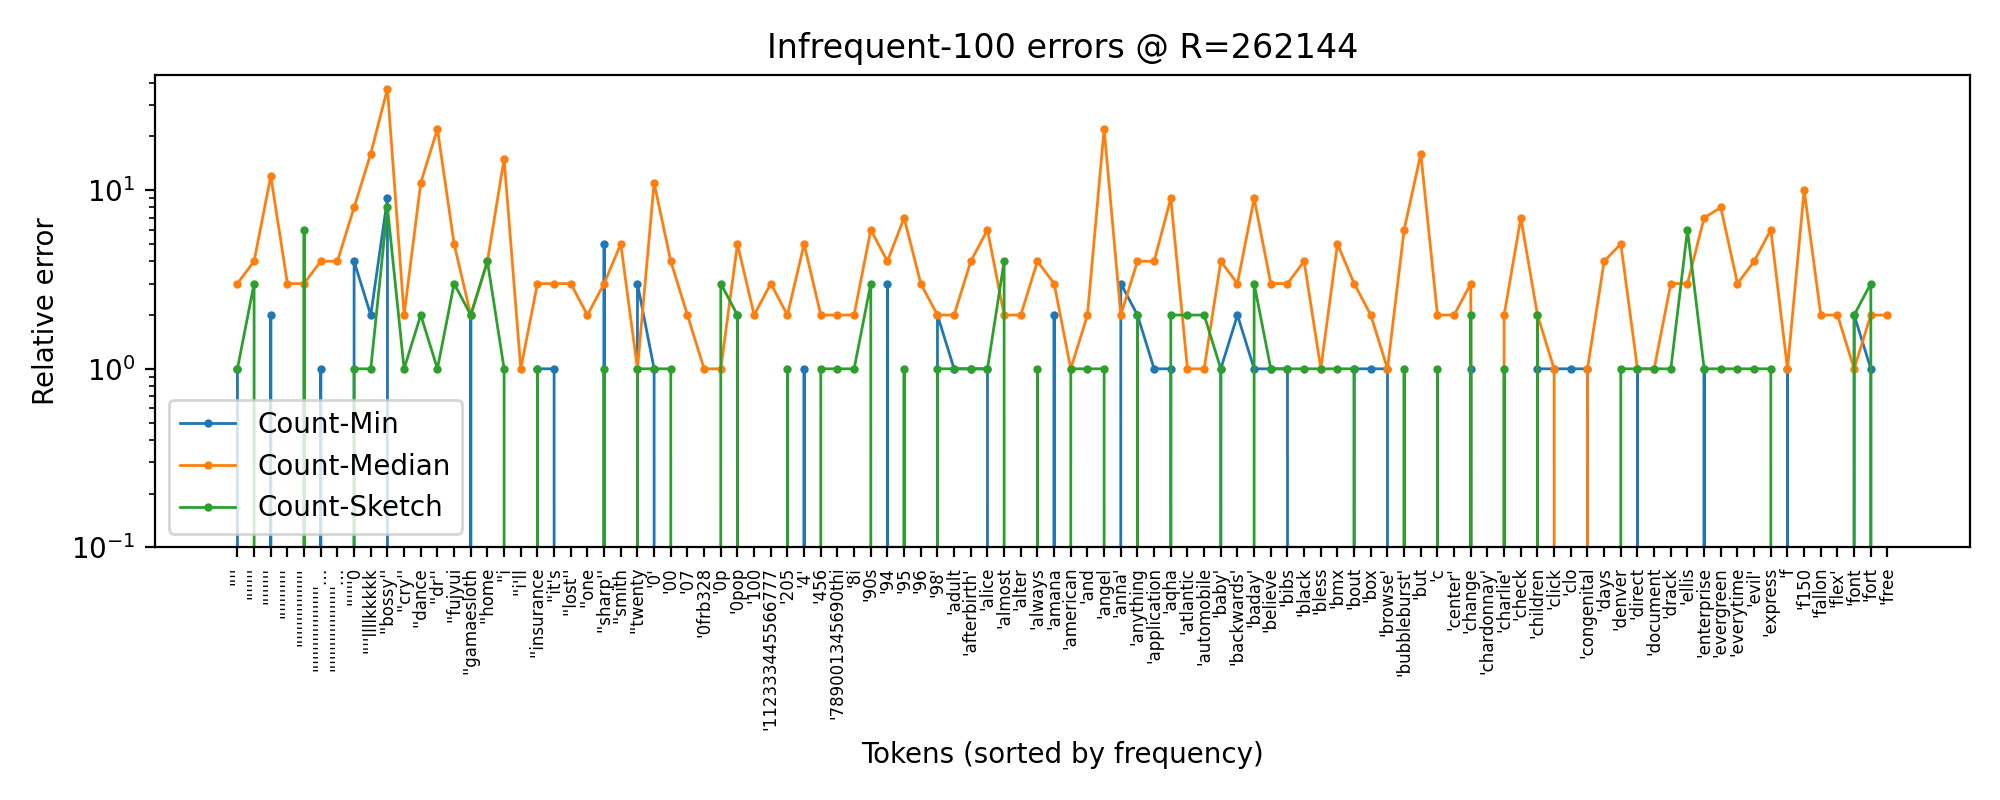
\includegraphics[width=\linewidth]{../outputs/a2/errors_R262144_Infrequent_100.png}
    \caption{Infrequent-100}
  \end{subfigure}
  \caption{Relative-error curves for $R=2^{18}$.}
  \label{fig:error-r262144}
\end{figure}


\begin{itemize}
  \item With the widest sketches, all medians drop to zero and the error curves flatten, indicating the structures now recover the true counts on almost every probe (Table~\ref{tab:median-trends}, bottom block).
  \item Residual deviations (Figure~\ref{fig:error-r262144}) stem from the few tokens that still hash-collide; the signed nature of Count-Sketch keeps its spikes smallest whenever they appear.
\end{itemize}


\begin{figure}[H]
  \centering
  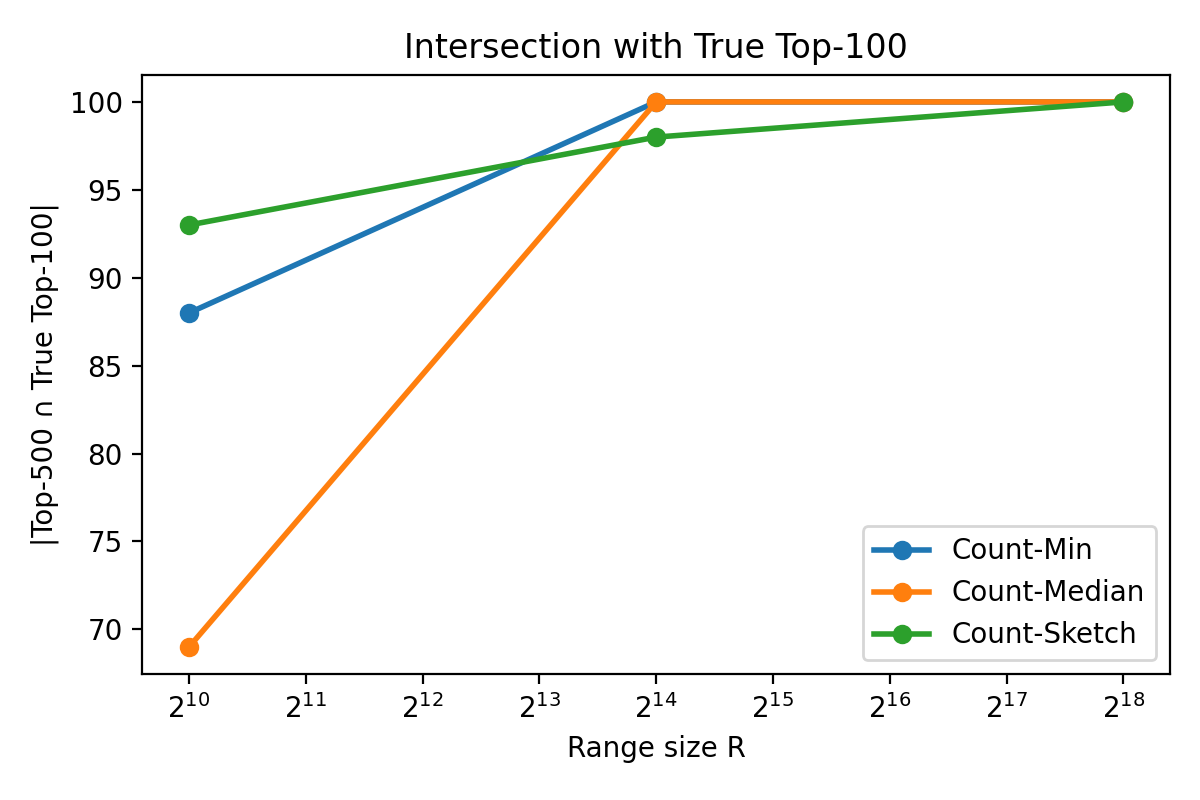
\includegraphics[width=0.55\linewidth]{../outputs/a2/top500_intersection.png}
  \caption{Intersection size of sketch top-500 with true top-100 across $R$.}
 \label{fig:top500}
\end{figure}


\begin{table}[H]
  \centering
  \begin{tabular}{lccc}
\toprule
Sketch & $R=2^{10}$ & $R=2^{14}$ & $R=2^{18}$ \\
\midrule
\multicolumn{4}{c}{Frequent-100 median relative error} \\
\midrule
Count-Min & 0.357 & 0.007 & 0 \\
Count-Median & 0.578 & 0.016 & 0 \\
Count-Sketch & 0.072 & 0.002 & 0 \\
\addlinespace
\midrule
\multicolumn{4}{c}{Random-100 median relative error} \\
\midrule
Count-Min & 3127.75 & 46 & 0 \\
Count-Median & 4764 & 109.5 & 1.5 \\
Count-Sketch & 1 & 1 & 0.417 \\
\addlinespace
\midrule
\multicolumn{4}{c}{Infrequent-100 median relative error} \\
\midrule
Count-Min & 4145 & 79 & 0 \\
Count-Median & 7008.5 & 196.5 & 3 \\
Count-Sketch & 1 & 1 & 1 \\
\bottomrule
\end{tabular}
  \caption{Median relative errors across sketch families and $R$.}
  \label{tab:median-trends}
\end{table}






\section{Top-500 Intersection}
The heap-based tracker yields the set intersection sizes summarised in Table~\ref{tab:intersection}. Small values of $R$ drop many true heavy hitters, while widening to $R=2^{14}$ markedly improves overlap for every sketch in this sample.

\begin{table}[H]
  \centering
  \begin{tabular}{lccc}
\toprule
Sketch & $R=2^{10}$ & $R=2^{14}$ & $R=2^{18}$ \\
\midrule
Count-Min & 88 & 100 & 100 \\
Count-Median & 69 & 100 & 100 \\
Count-Sketch & 93 & 98 & 100 \\
\bottomrule
\end{tabular}
  \caption{Size of $\text{Top-500}_{\text{sketch}} \cap \text{Top-100}_{\text{truth}}$.}
  \label{tab:intersection}
\end{table}

\section{Reproducibility Checklist}
\begin{itemize}
  \item \textbf{Generate outputs}: \verb|python main_a2.py|\ 
  \item \textbf{Artifacts}: Plots land in \texttt{outputs/a2/} with filenames \texttt{errors\_R\{R\}\_\{category\}.png} and \texttt{top500\_intersection.png}; metrics appear in \texttt{outputs/a2/summary.json}. Each run also writes \texttt{error\_table.tex}, \texttt{median\_table.tex}, and \texttt{run\_summary.tex} so the report stays numerically consistent with the latest metrics—no manual edits required.
\end{itemize}

\section{Conclusions}
The combined pipeline is structured to stream the AOL log once, maintain exact frequencies for evaluation, compare three sketches at multiple width settings, quantify relative errors for representative token buckets, and evaluate top-$k$ recovery. Count-Min offers deterministic upper bounds but needs wider tables to suppress overestimation on sparse items. Count-Median remains positively biased because it averages unsigned counters, yet its variance shrinks quickly as $R$ grows. Count-Sketch leverages signed updates to curb both bias and variance, delivering the tightest estimates once the width is large enough.


\end{document}
